% !TeX root = ../thuthesis-example.tex

\chapter{实验}
\label{chp:exp}

接下来,我们通过实验对本文提出的方法进行评测,主要关注以下几个问题:

\begin{itemize}
    \item 本文工作可以收集到多少调用记录,从中可以构建多少具体算子?文中提出的偏算子与分类规则,是否能够支持简单的符号规则与约束的自动推导算法?
    \item 对于引入具体算子后的混合算子计算图生成算法,其能否高效地生成合法的计算图,以产生供测试所用的模型?
    \item 基于混合算子计算图生成的模糊测试,其是否在代码分支覆盖率上得到了提升?
    \item 对于本文改进后的模糊测试框架,其是否能够寻找到漏洞?这些漏洞是否可以被前人工作发掘,其质量与实际意义如何?
\end{itemize}

\section{实验设置}

在测试对象上,我们选取了当前最流行的两种深度学习框架 TensorFlow 与 PyTorch 中的编译器。
在与类似工作的比较上,我们主要选择目前效果最好的计算图层面模糊测试框架, NNSmith 。
在实验环境上,我们使用一台 CPU 为 AMD Ryzen Threadripper PRO 5975WX 32-Cores ,内存有 256 GB (3200 MHz),磁盘为 4TB PCIe-4 NVMe SSD ,操作系统为 Ubuntu 22.04.2 LTS 的工作站。
对于算子收集、计算图生成、覆盖率统计实验,我们只考虑在 CPU 上使用 TensorFlow XLA 编译器和 PyTorch JIT 编译器的情况。而在寻找漏洞时,我们包括了在 GPU 上的编译与运行,并引入了两种框架中的其它编译器。

为了统计分支覆盖率,我们需要对深度学习框架进行重新编译。
我们参考 NNSmith 仓库里的覆盖率实验指导\cite{nnsmith_expinstr}进行编译。
对于 PyTorch 框架,我们使用 Clang-14 以及其附带的基于源码的覆盖率统计工具\cite{clang14_cov}编译其 \texttt{2.1.0a0+git6c934a8} 版本。我们较为保守地对可能与 JIT 相关的源码都进行插桩以统计覆盖率。 PyTorch 中与 JIT 相关的代码分散在各处而没有清晰的界限,因此我们粗略地包括了 \texttt{pytorch/csrc} 与 \texttt{aten} 文件夹下的代码。
对于 TensorFlow 框架,我们使用 GCC-9.4 和覆盖率统计工具 GCOV\cite{gcov} 编译其 2.12 开发版 (git hash 前缀为 \texttt{5a6fc0})。我们只对其源码中 \texttt{tensorflow/compiler} 文件夹下的代码进行插桩以统计覆盖率。

\section{具体算子收集}

\begin{table}[]
\centering
\caption{数据收集与整理情况}
\label{tab:opstat}
\begin{tabular}{ccccc}
  \toprule
             & \makecell{收集到轨迹的接口 /\\被插桩接口} & 不重复轨迹 & \makecell{具体算子 /\\具体算子对应的接口} & \makecell{偏算子} \\ \midrule
  PyTorch    & 841 / 1321           & 63144   & 29083 / 678          & 5823  \\
  TensorFlow & 316 / 423            & 34228   & 12908 / 214          & 1799  \\ \bottomrule
\end{tabular}
\end{table}

首先,我们启用 \ref{sec:collect} 中所述的对深度学习框架接口的插桩,按照各自的文档分别运行 PyTorch 的单元测试\cite{pytorch_tests}和 TensorFlow 的单元测试\cite{tf_tests, tf_doctests},从而收集调用轨迹。
表 \ref{tab:opstat} 展示了在插桩、收集、和构建算子过程中的关键数据。

对于 PyTorch ,在全部被插桩的 1323 个接口中,有 841 个(64\%)接口收集到了至少一个调用轨迹; TensorFlow 的这一数值为 316 (75\%)。
二者接口数相差甚远,是因为在 PyTorch 中,有很多“孪生接口”,如 \texttt{Tensor.add} 与它的“就地更改”版本 \texttt{Tensor.add\_} ;还有互为别名的接口,如 \texttt{torch.abs} 与 \texttt{torch.absolute} 。 TensorFlow 中也有类似接口,如 \texttt{tf.raw\_ops.Concat} 与另一个版本 \texttt{tf.raw\_ops.ConcatV2} ,但这种重复与冗余相较 PyTorch 较少。此外, PyTorch 中存在一些复合接口,如 \texttt{Tensor.addbmm} ,而 TensorFlow 中没有这类复合算子。
两个框架均有一部分接口没有收集到任何调用轨迹,很大程度上是因为相互类似的接口的存在。如 \texttt{torch.abs} 被收集到了很多调用轨迹,而 \texttt{torch.absolute} 则没有任何调用轨迹;又如 \texttt{tf.raw\_ops.ConcatV2} 收集到了调用轨迹,而 \texttt{tf.raw\_ops.Concat} 没有。

可以发现,应用 \ref{sec:build_cop} 中的筛选规则后,超过一半的轨迹被丢弃,这主要是因为类似 \texttt{torch.rand\_like} 的接口在单元测试中被大量调用,但不满足确定性要求。根据表中具体算子对应原框架接口的数量可知,分别有 19\% (PyTorch)/ 32\% (TensorFlow)的接口无法通过这一步中的两条检查规则。

最后,应用 \ref{sec:partialop} 中对具体算子的分类规则,可以分别建立 5823 (PyTorch)/ 1799 (TensorFlow)个供符号规则与约束自动推导算法使用的偏算子。基于这些偏算子,外部合作者实现了仅支持加、减、乘、除、最大、最小和模运算的推导算法,就可以为 76\% (PyTorch)/ 84\% (TensorFlow)的偏算子推导出规则与约束。若某接口至少有一个偏算子推导成功就认为这个接口推导成功,则这部分接口占偏算子对应的全部接口的 91\% (PyTorch) / 90\% (TensorFlow) 。若推导成功的接口以符号化算子的形式在混合算子计算图生成中被合法地使用了至少一次就认为对该接口的推导有效,则推导有效的接口占全部参与计算图生成的接口的 96\% (PyTorch) / 96\% (TensorFlow)。可见,本文提出的偏算子概念可以帮助自动推导算法取得较好的效果。

\section{模糊测试用例生成与分支覆盖率}
\label{sec:exp_gen}

对于测例生成,我们比较以下三种不同的计算图生成算法:
\begin{itemize}
    \item NNSmith 中的完全符号化生成算法,记为 NNSmith 。
    \item 同时引入了 NNSmith 中的符号化算子与本文工作中的具体算子的混合算子计算图生成算法,记为 HybridGen-r 。
    \item 利用外部合作者在偏算子上的推导结果,将推导成功的偏算子符号化;在 HybridGen-r 的基础上,保留具体算子的同时,加入这部分通过自动推导建立的符号化算子,进行混合算子计算图生成,记为 HybridGen 。
\end{itemize}
我们限定生成测例的总时间为 4 小时,与前人工作\cite{nnsmith,tzer}保持一致。从后续实验可以看出, 4 小时足够让实验结果基本收敛。

首先,我们考虑如何选取计算图的大小,即图中算子的数量。
图 \ref{fig:covexp:size} 为 HybridGen 算法在 PyTorch 上的消融实验,评价指标(纵轴)为覆盖率,节点数目分别为 1、5、9、13 ,4 小时内每种节点数下生成的合法模型数量标注在图例中。
可以看出,过小的计算图(如单算子计算图)虽然生成速度很快,但会因为无法触发编译器中的图层面优化逻辑(如多算子融合)而只能达到较低的覆盖率,这体现了图层面的模糊测试相比单算子模糊测试的优越性;但计算图大小在增长到一定程度后再继续增大则对提高覆盖率无益,这主要是因为编译器中的优化逻辑一般只涉及到局部几个算子,而不会对较大的子图做优化。
由于目前没有实现在保证漏洞可复现的同时最小化测例的算法,对于较大的计算图构成的测例,发现漏洞后人工进行最小化时的工作量较大。
所以,我们最终选取 5 作为计算图的大小来进行后续实验,以平衡覆盖率效果与人工调试的难度。

其次,我们考察测例生成的效率。
在这一步,我们使用没有为了统计分支覆盖率而在编译时进行插桩的深度学习框架。这是因为在真实场景中进行模糊测试的目的是为了寻找漏洞,而不需要统计分支覆盖率指标,因此只需用官方预编译的普通版本即可。所以在此我们排除插桩带来的额外开销,以反映真实场景中测例生成的效率。
大部分情况下,从一个计算图可以建立一个深度学习模型,从而生成一个测例。但由于在生成计算图时,我们只对张量形状与数据类型做了匹配,而没有考虑输入张量的数值对于算子的合法性,因此会有少量计算图无法被构建为合法的深度学习模型,从而形成一个合法测例。
对此,我们使用解释执行的方式来判断合法性:如果一个计算图对应的模型可以在不启用编译器的解析执行模式下运行成功,则我们认为该计算图合法。
表 \ref{tab:num_tests} 呈现了不同算法在 4 小时内生成的计算图的数量与合法率。
从中可以看出,完全符号化的生成算法 NNSmith 速度最快,且合法率最高。引入了大量具体算子的 HybridGen-r 算法生成速度变慢,且合法率略微下降。这是因为 NNSmith 算法只需考虑 70 余种算子,而 HybridGen-r 算法需要额外考虑上万种具体算子如何被合法地插入计算图,因而时间开销更大;且由于算子种类更多样,合法性更难以保证。至于进一步引入了大量基于自动推导建立的符号算子的 HybridGen 算法,其需要考虑更多算子,且推导出的规则不一定完全正确,因此生成速度与合法性均进一步下降。

\begin{table}[]
\centering
\caption{测例生成情况}
\label{tab:num_tests}
\begin{tabular}{ccccc}
  \toprule
  \multirow{2}{*}{} & \multicolumn{2}{c}{TensorFlow} & \multicolumn{2}{c}{PyTorch} \\ \cmidrule(lr){2-3} \cmidrule(lr){4-5} 
                    & 计算图数量        & 合法率             & 计算图数量      & 合法率            \\ \midrule
  NNSmith           & 139287       & 100.0\%      & 639437     & 100.0\%     \\
  HybridGen-r       & 134120       & 98.1\%      & 410607     & 99.8\%     \\
  HybridGen         & 108572       & 94.8\%      & 208693     & 98.9\%     \\ \bottomrule
\end{tabular}
\end{table}

然后,我们分别在两种框架上对三种计算图生成算法进行源码分支覆盖率评测,以比较不同算法所生成测例的多样性,和基于它们的模糊测试对目标测试的充分程度。
在具体实现上,我们用自编译的为了统计覆盖率而进行了插桩的深度学习框架,对上一步实验中在 4 小时内生成的所有测例用编译执行模式进行重放。
图 \ref{fig:covexp} 表明,在两种框架上, HybridGen-r 均能显著超过 NNSmith ,提升幅度达 13.5\% (PyTorch) / 20.9\% (TensorFlow),证明了引入具体算子做计算图生成的有效性。
而对于将具体算子抽象化以提高张量形状多样性的 HybridGen ,则可以进一步提高分支覆盖率,相较 NNSmith 提升幅度达 14.9\% (PyTorch) / 23.5\% (TensorFlow),相较 HybridGen-r 提升幅度达 1.3\% (PyTorch) / 2.2\% (TensorFlow) ,证明了偏算子这一概念可以支撑自动推导算法使深度学习框架与编译器的模糊测试更加充分,为未来工作提供了实现基础与想象空间。

\begin{figure}
    \centering
    \subcaptionbox{PyTorch\label{fig:covexp:pt}}
        {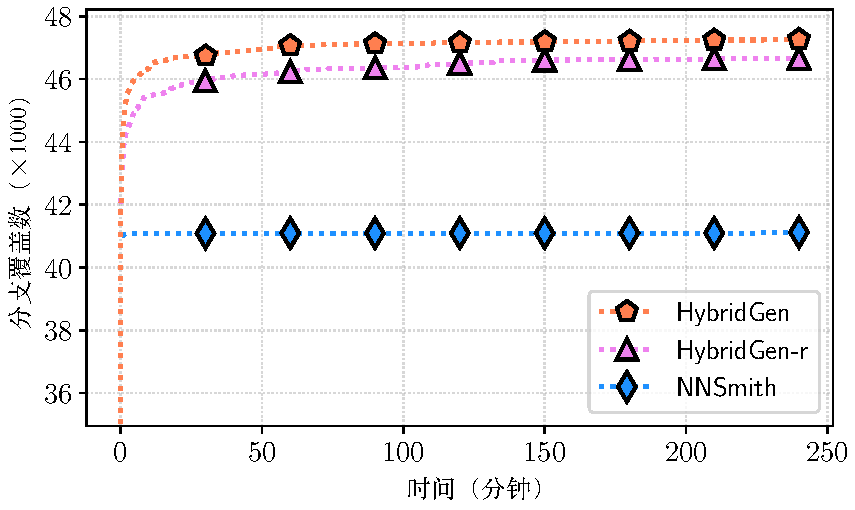
\includegraphics[width=0.48\linewidth]{figures/pt_cov.pdf}}
    \subcaptionbox{TensorFlow\label{fig:covexp:tf}}
        {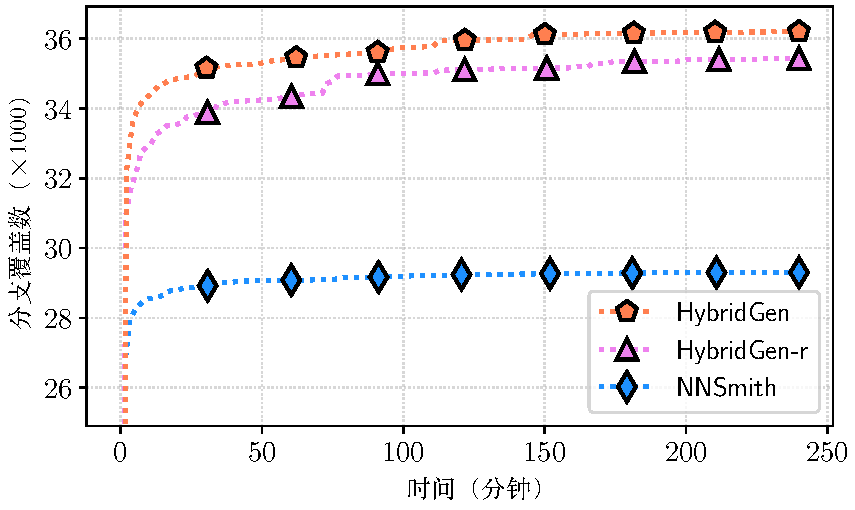
\includegraphics[width=0.48\linewidth]{figures/tf_cov.pdf}}
    \subcaptionbox{模型大小的影响\label{fig:covexp:size}}
        {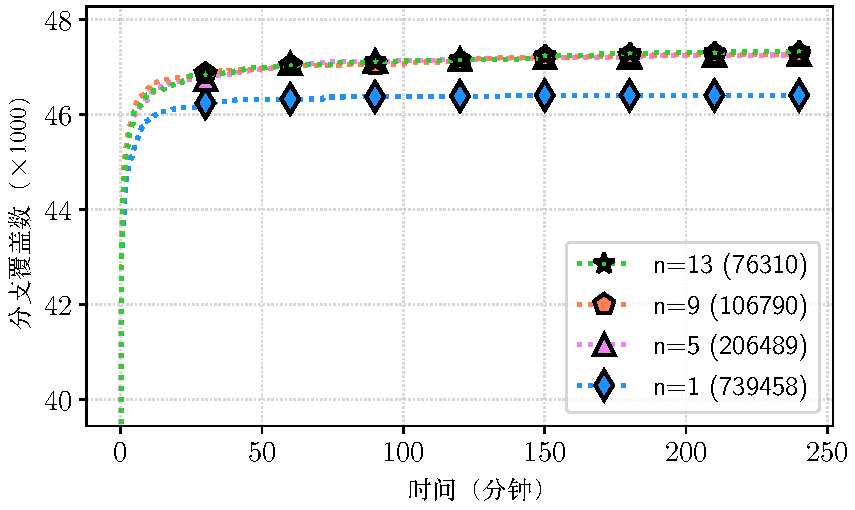
\includegraphics[width=0.48\linewidth]{figures/size_cov.pdf}}
    \caption{模糊测试 4 小时的分支覆盖率变化}
    \label{fig:covexp}
\end{figure}

% PyTorch:
% ----> max cov 41120.0 + max tests 639500
% ----> max cov 46654.0 + max tests 409900  1.1345817121
% ----> max cov 47266.0 + max tests 206500  1.1494649805, 1.0131178463
% TF:
% ----> max cov 29303.0 + max tests 140000
% ----> max cov 35426.0 + max tests 132000  1.2089547145
% ----> max cov 36203.0 + max tests 109000  1.2354707709, 1.0219330435
% Size:
% ----> max cov 46404.0 + max tests 739500
% ----> max cov 47266.0 + max tests 206500
% ----> max cov 47275.0 + max tests 106800
% ----> max cov 47332.0 + max tests 76400

\section{漏洞寻找}

我们分别在以下设置上运行模糊测试,以寻找潜在漏洞。

\begin{itemize}
    \item TensorFlow: XLA 编译器(包括 CPU 、 GPU)、 TFLite (只支持 CPU);
    \item PyTorch: JIT 编译器、 PyTorch 2.0 编译接口(包括 TorchDynamo 和 TorchInductor)(均包括 CPU 、 GPU)。
\end{itemize}

\subsection{效果概述}

通过不断运行模糊测试框架,并辅以人工筛选与检查,目前我们在开源代码平台 GitHub 上共计向两种框架提交了 76 个被开发团队确认的漏洞。表 \ref{tab:bugs} 从开发团队对漏洞的跟进情况和漏洞的症状两方面进行了统计。
其中, TensorFlow 团队对我们提交的漏洞修复意愿较低,大部分漏洞在确认之后的半年甚至更长时间都没有后续跟进,因而我们逐渐将工作重点放在挖掘 PyTorch 的漏洞上,所以两种框架漏洞总数的差异并不能反映二者可靠性的关系。
对于 PyTorch ,由于开发团队在 2022 年 12 月发布 PyTorch 2.0 后逐渐将工作重点放在了 TorchDynamo 和 TorchInductor 组成的编译技术栈上,而对修复 JIT 编译模块对积极性不强,因此我们在寻找漏洞时也跟随了这一调整。

从表 \ref{tab:bugs} 前 3 列可知,我们提交的绝大部分漏洞都受到了开发者的认可,只有极少数漏洞开发者表示不会进行修复。
对于 PyTorch 团队近期的工作重心 PyTorch 2.0 中的编译技术栈,我们提交的大部分(80.5\%)均已被修复,说明我们提交的漏洞受到重视,具有较高的重要性。
PyTorch 的核心开发者之一在 GitHub 上对我们的工作给予了认可与赞赏,引其原文\cite{ngimel_comments}如下。其表达的主要意思为,我们提交的漏洞并非故意构造而在现实中难以遇到,而是发现了一些可以轻易在实践中被触发,却没有被开发者维护的测试集覆盖的情形。
这段评价不仅体现了本文工作可以生成较为多样的测例,以弥补人工编写的测例集的不足,而且说明了我们构造的测例是在实践中常见的情形,从而具有实际意义。事实上,这两点优势主要均来自于我们在收集具体算子时对真实世界中现有代码的充分利用。

\begin{shadequote}
\small
That said, the bugs you've reported are \textit{high quality}, and as you say, don't look like specially fuzzed set that's impossible to see in practice. They \textit{did} reveal a few common themes that are easy to encounter in practice (even if they are not in our common testing/benchmarking suite), like inplace ops handling (we are working on that), or cpu codegen errors caused by improper use of \texttt{\_\_restrict\_\_} (also working on that).
\end{shadequote}

从表 \ref{tab:bugs} 后 3 列可知,在我们寻找到的漏洞中,报错与错误输出的情况占大多数,而进程崩溃占少数。其中,
“报错”指模型在编译或执行的过程中失败,进程以触发 Python 异常的方式结束;
“错误输出”指模型可以顺利编译与执行,但在没有任何报错的情况下,编译执行模式的输出与解释执行不一致,这在实际应用中可能导致模型在编译之后无法达到先前的效果;
而“进程崩溃”指模型在编译或执行的过程中,进程以非正常的方式结束,如被操作系统强制终止等。
相较“报错”与“进程崩溃”,“错误输出”难以引起用户的注意,因此发现此类漏洞对提升深度学习系统的可靠性具有较强的现实意义。

\begin{table}[]
\centering
\caption{漏洞挖掘情况}
\label{tab:bugs}
\begin{tabular}{ccccccc}
  \toprule
                  & 总计 & 已修复 & 不修复 & 报错                  & 错误输出                & 进程崩溃               \\ \midrule
  PyTorch JIT     & 21 & 8   & 2   & \multirow{2}{*}{39} & \multirow{2}{*}{19} & \multirow{2}{*}{4} \\
  PyTorch 2.0     & 41 & 33  & 0   &                     &                     &                    \\ \cmidrule(lr){1-7} 
  TensorFlow XLA  & 7  & 0   & 1   & \multirow{2}{*}{5}  & \multirow{2}{*}{7}  & \multirow{2}{*}{2} \\
  TensorFlow Lite & 7  & 0   & 0   &                     &                     &                    \\ \bottomrule
\end{tabular}
\end{table}

接下来,我们呈现两个具体漏洞,展示它们的症状表现并分析其根因。

\subsection{底层代码漏洞举例}

PyTorch Issue \#93365\cite{pti93365}是我们提交的被开发团队标记为“high priority”(高优先级)的漏洞之一。
其症状表现为编译后的模型会给出错误的计算结果,具体如代码 \ref{listing:pti93365} 所示。函数 \texttt{fn} 被 PyTorch 2.0 编译后,其返回的第二个张量 \texttt{v1} 被错误地计算为全 0 。(该测例并非模糊测试框架直接给出的原测例,而是经过了后期人工简化,如删去不影响触发漏洞的无关变量和计算等,以便于定位根因。代码 \ref{listing:pti93365} 在原 Issue 的基础上又做了进一步简化,但保持了漏洞的可复现性与根因的一致性。)

\begin{listing}[]
    \caption{PyTorch Issue \#93365 复现代码及报错信息}
    \label{listing:pti93365}
\begin{minted}[
    fontsize=\small,
    linenos, mathescape, escapeinside=||,
    % texcomments,
    frame=lines,
    framesep=1.5mm,    
]{python}
import torch

p0 = torch.tensor([[4.9334, 5.5571]]) # (1, 2)

def fn():
    v7 = torch.cat([p0, p0], dim=0) # v7: (2, 2)
    v1 = torch.mul(v7, v7) # v1: (2, 2)
    return v7, v1

ret_eager = fn()
compiled = torch.compile(fn)
ret_compiled = compiled()

assert torch.allclose(ret_eager[0], ret_compiled[0])
# ^^^ no error
assert torch.allclose(ret_eager[1], ret_compiled[1])
''' ^^^ WRONG!
AssertionError: 
ret_eager[1] =    tensor([[24.3384, 30.8814],
                          [24.3384, 30.8814]])
ret_compiled[1] = tensor([[0., 0.],
                          [0., 0.]])
'''
\end{minted}
\end{listing}

通过追踪与分析开发团队的讨论与修复方式可知,该错误的根因来自底层 C++ 关键字 \texttt{\_\_restrict\_\_} 的错误使用,我们认为其属于底层代码漏洞。
具体来说,对于 Python 语言描述的包含两条 CPU 计算语句的函数 \texttt{fn} , PyTorch 2.0 会将其编译为一个 C++ 语言实现的底层核函数 \texttt{kernel} ,如代码 \ref{listing:pti93365_cpp} 所示。
(我们在代码中添加了注释,以解释 C++ 层面的变量与计算和 Python 层面的变量与计算之间的对应关系。)
% 首先,该段代码通过两个 \texttt{for} 循环计算 Python 中的 \texttt{cat} 操作,将结果输出至 Python 变量 \texttt{v7} 在 C++ 层面对应的两个数组 \texttt{out\_ptr0} 和 \texttt{out\_ptr1} ,这两个数组各自存储了 \texttt{v7} 的一半数据。
% 其次,该段代码用一个 \texttt{for} 循环计算 Python 中的 \texttt{mul} 操作;输入为数组 \texttt{in\_ptr2} ,对应 Python 中 \texttt{v7} 的全部,而输出为数组 \texttt{out\_ptr2} ,对应 Python 中的 \texttt{v1} 。
分析代码可以发现, Python 层面的两个操作存在数据依赖,即 \texttt{mul} 操作的输入 \texttt{v7} 是前一个 \texttt{cat} 操作的输出。而表现在 C++ 层面, \texttt{mul} 操作的输入为 \texttt{in\_ptr2} ,似乎并非 \texttt{cat} 操作的输出 \texttt{out\_ptr0} 与 \texttt{out\_ptr1} 。
然而实际上, \texttt{out\_ptr0} 指向的是 \texttt{v7} 的前一半数据, \texttt{out\_ptr1} 指向的是 \texttt{v7} 的后一半数据,而 \texttt{in\_ptr2} 指向的是 \texttt{v7} 的全部数据,即 \texttt{out\_ptr0} 和 \texttt{out\_ptr1} 均与 \texttt{in\_ptr2} 发生了数据重叠。
而 C++ 函数的参数列表中,被 \texttt{\_\_restrict\_\_} 关键字标记的指针会被编译器认为不存在“别名”,即该指针指向的内存区域不会被其它名称的指针所指并修改,从而可以优化访存逻辑以提高性能。
PyTorch 的开发者在此过于激进地使用了这一优化,导致 \texttt{\_\_restrict\_\_} 关键字的含义与 \texttt{in\_ptr2} 指向的区域被 \texttt{out\_ptr0} 和 \texttt{out\_ptr1} 所指并发生了修改的实际情况不一致,因此产生了错误。

\begin{listing}[]
    \caption{PyTorch Issue \#93365 复现代码}
    \label{listing:pti93365_cpp}
\begin{minted}[
    fontsize=\small,
    linenos, mathescape, escapeinside=||,
    % texcomments,
    frame=lines,
    framesep=1.5mm,    
]{cpp}
extern "C" void kernel(const float* __restrict__ in_ptr0, // p0
                       const float* __restrict__ in_ptr1, // p0
                       const float* __restrict__ in_ptr2, // v7
                       float* __restrict__ out_ptr0, // v7 的前一半
                       float* __restrict__ out_ptr1, // v7 的后一半
                       float* __restrict__ out_ptr2) // v1
{
    { // cat 计算的一部分:将 p0 中的值复制到 v7 的前一半
        #pragma GCC ivdep
        for(long i0=0; i0<2; i0+=1)
        {
            auto tmp0 = in_ptr0[i0];
            out_ptr0[i0] = tmp0;
        }
    }
    { // cat 计算的一部分:将 p0 中的值复制到 v7 的后一半
        #pragma GCC ivdep
        for(long i0=0; i0<2; i0+=1)
        {
            auto tmp0 = in_ptr1[i0];
            out_ptr1[i0] = tmp0;
        }
    }
    { //  mul 计算:将 v7 与 v7 做元素级相乘,输出至 v1
        #pragma GCC ivdep
        for(long i0=0; i0<4; i0+=1)
        {
            auto tmp0 = in_ptr2[i0];|\label{listing:pti93365_cpp:inptr2}|
            auto tmp1 = tmp0 * tmp0;
            out_ptr2[i0] = tmp1;
        }
    }
}
\end{minted}
\end{listing}

下降到汇编层面上分析,若使用 \texttt{\_\_restrict\_\_} 关键字,则在 X86 平台上编译器可以将代码 \ref{listing:pti93365_cpp} 编译为代码 \ref{listing:pti93365_asm} 所示的汇编指令。前 3 条指令将 \texttt{in\_ptr0} 、 \texttt{in\_ptr1} 、 \texttt{in\_ptr2} 指向的数组从内存分别加载至寄存器,第 4 条指令将 \texttt{in\_ptr0} 的数据写入 \texttt{out\_ptr0} ,第 5 条指令将 \texttt{in\_ptr1} 的数据写入 \texttt{out\_ptr1} ,第 6 条指令将 \texttt{in\_ptr2} 的数据与自己相乘,然后在第 7 条指令将结果存入 \texttt{out\_ptr2} 。
其错误在于,第 4 、 5 条指令实际上修改了第 6 条指令的输入,因此 \texttt{in\_ptr2} 数组需要在做乘法之前重新加载。但 \texttt{\_\_restrict\_\_} 关键字使编译器认为 \texttt{in\_ptr2} 指向的内存区域不会被修改,因此没有加载修改后的值,而是直接使用了之前向寄存器中加载的被修改以前的值。
由于在实际中 \texttt{in\_ptr2} 指向的内存经常为初始值 0 ,因此运行该测例时进行乘法之后的输出也常常为 0 ,产生错误输出。

对于该漏洞,开发者的修复方案为,在编译器 TorchInductor 生成底层 C++ 代码的逻辑中,不向函数参数列表中的指针添加 \texttt{\_\_restrict\_\_} 关键字,通过牺牲潜在的性能提升以保证正确性。

此案例说明,本文工作虽然从上层 Python 接口层面进行模糊测试,但可以寻找到根因位于底层 C++ 代码中的漏洞。
而该漏洞需要两个算子产生数据依赖以触发,体现了在多算子计算图层面进行模糊测试的意义。

\begin{listing}[]
    \caption{代码 \ref{listing:pti93365_cpp} 的一种可能的汇编实现}
    \label{listing:pti93365_asm}
\begin{minted}[
    fontsize=\small,
    linenos, mathescape, escapeinside=||,
    % texcomments,
    frame=lines,
    framesep=1.5mm,    
]{nasm}
movq      (%rdi), %rax      ; auto tmpx = in_ptr0[:]
movq      (%rsi), %r10      ; auto tmpy = in_ptr1[:]
movups    (%rdx), %xmm0     ; auto tmp0 = in_ptr2[i0];
movq      %rax, (%rcx)      ; out_ptr0[:] = tmpx;
movq      %r10, (%r8)       ; out_ptr1[:] = tmpy;
mulps     %xmm0, %xmm0      ; auto tmp1 = tmp0 * tmp0;
movups    %xmm0, (%r9)      ; out_ptr2[:] = tmp1;
retq
\end{minted}
\end{listing}

\subsection{高层代码漏洞举例}

PyTorch Issue \#95181\cite{pti95181}同样是我们为 PyTorch 2.0 编译技术栈寻找到的漏洞之一,而其根因位于整个编译流程的 Python 实现中,因此我们认为其属于高层代码漏洞。
原测例经人工简化后如代码 \ref{listing:pti95181} 所示,只需单个算子即可触发。其症状表现为,编译 \texttt{fn} 函数会失败,并产生报错信息如代码最后的注释所示。

\begin{listing}[]
    \caption{PyTorch Issue \#95181 复现代码及报错信息}
    \label{listing:pti95181}
\begin{minted}[
    fontsize=\tiny,
    linenos, mathescape, escapeinside=||,
    % texcomments,
    frame=lines,
    framesep=1.5mm,    
]{python}
import torch

def fn(x: torch.Tensor):
    return x.sub(other=1, alpha=2)

x = torch.rand([1], dtype=torch.float64) |\label{listing:pti95181:x}|

ret_eager = fn(x)
compiled = torch.compile(fn)
ret_compiled = compiled(x)
''' ^^^
Traceback (most recent call last):
  File "python3.10/site-packages/torch/_dynamo/utils.py", line 1196, in run_node
    return getattr(args[0], node.target)(*args[1:], **kwargs)
  File "python3.10/site-packages/torch/utils/_stats.py", line 20, in wrapper
    return fn(*args, **kwargs)
  File "python3.10/site-packages/torch/_subclasses/fake_tensor.py", line 989, in __torch_dispatch__
    return self.dispatch(func, types, args, kwargs)
  File "python3.10/site-packages/torch/_subclasses/fake_tensor.py", line 1172, in dispatch
    r = func(*args, **kwargs)
  File "python3.10/site-packages/torch/_ops.py", line 284, in __call__
    return self._op(*args, **kwargs or {})
  File "python3.10/site-packages/torch/_prims_common/wrappers.py", line 220, in _fn
    result = fn(*args, **kwargs)
  File "python3.10/site-packages/torch/_prims_common/wrappers.py", line 130, in _fn
    result = fn(**bound.arguments)
  File "python3.10/site-packages/torch/_refs/__init__.py", line 1608, in sub
    return prims.sub(a, b)
  File "python3.10/site-packages/torch/_ops.py", line 284, in __call__
    return self._op(*args, **kwargs or {})
  File "python3.10/site-packages/torch/_prims/__init__.py", line 341, in _elementwise_meta
    utils.check_same_dtype(*args)
  File "python3.10/site-packages/torch/_prims_common/__init__.py", line 1079, in check_same_dtype
    raise RuntimeError(msg)
RuntimeError: Tensor with dtype torch.float32 is not the expected dtype of torch.float64!
'''
\end{minted}
\end{listing}

通过分析报错信息中的调用栈可知,其触发过程分为以下几步:

\begin{enumerate}
    \item 在代码 \ref{listing:pti95181} 第 25 行所指的源码附近,测例中的 Python 内置整型参数 \texttt{b} 被提升为了 Python 内置浮点型。\cite{torch_promarg}
    \item 在代码 \ref{listing:pti95181} 第 27 行所指的源码函数中, \texttt{b} 被更新为其与系数 \texttt{alpha} 的乘积,通过 \texttt{prims.mul(b, alpha)} 实现,其返回值类型是数据类型为 \texttt{float32} 的 PyTorch 张量。\cite{torch_primmul}
    \item 代码 \ref{listing:pti95181} 第 27 行所指的源码函数最后执行 \texttt{prims.sub(a, b)} 以计算最终结果。\cite{torch_primsub}此处传入的参数 \texttt{a} 是数据类型为 \texttt{float64} 的 PyTorch 张量(由于我们在代码 \ref{listing:pti95181} 第 \ref{listing:pti95181:x} 行生成的输入为此类型),与上一步更新后的 \texttt{b} 类型不一致。但在 \texttt{prims.sub} 中,对于两个输入参数均为 PyTorch 张量的情况,有强制数据类型一致性检查,因此编译失败而报错。
\end{enumerate}

对于该错误,开发者最终的修复方案为,在上述第 2 步中,若 \texttt{b} 不是 PyTorch 张量类型,则用语句 \texttt{b = b * alpha} 将其与系数 \texttt{alpha} 相乘,以保持其非 PyTorch 张量类型,而把提升类型至 PyTorch 张量的任务交给 \texttt{prims.sub} 接口,以规避报错。\cite{pti95181_fix}

在此案例中,计算操作 \texttt{x.sub(other=1, alpha=2)} 的用法来自于收集到的具体算子。
对于 NNSmith ,其虽然以符号化的形式将 \texttt{sub} 加入到了算子集合中,但只考虑了 \texttt{other} 参数为张量的用法,因而无法生成该测例以触发由类型提升过程导致的错误。
而本文工作中收集到了 \texttt{other} 参数为 Python 内置整型的用法,将其视为算子的非张量属性参数之一而固定不变,只考虑张量 \texttt{x} 的合法性匹配,因而能够生成此测例。
这体现了对于用法灵活的深度学习框架接口,从真实世界代码中收集多样的常见用法并将其引入模糊测试的用例生成,相比纯粹符号化建模算子的方法可以找到更多漏洞,并且具有较强的实际意义。
